\subsection{Währenddessen im Zoo}
\label{sec:Kap-6.3.3}

war die AG Domänenmodelleirmg auch nicht untätig

Während die AG Entwicklungsplanung mit Visionen und Stakeholdern beschäftigt ist (s. Kap), hat die AG Domänenmodellierung schon Fortschritte gemacht , mittlerweile sind die Zusammenhänge Tier tierpflger Vertrtung deutlicher geworden

- Jetzt wo das Futterbestell Projekte Formen annimmt soll sich die AG das angucken
weitmöglichste automatisierung aller fütternugstätigkeiten dazu gehört auch futter bestellen, lagerverwaltung etc

Wer bestellt Futter, wo wird das bestellt, wie passiert die Lieferung, wo wird das gelagert, wie lange im voraus muss bestellt werden



versucht die AG Domänenmodellierung die Zusammenhänge zwischen x und y ...zu durchdirngen


AG Domänenmodellierung, Tier Tiepfleger füttern, Gehege säubern etc.
- mehrere AF Diagramme der unterschiedlichen Tierpfleger
- ein Klassendiagramm der Tierarten


- Aktivitätsdiagramm



- auch was mit Produkt







% ab hier alt

\textbf{Ausschnitt aus den Gesprächsnotizen:}
\begin{itemize}[
	label={\raisebox{-2mm}{
\includegraphics[scale=0.8]{Bilder/speech_balloon_green.pdf}}},
	leftmargin=12mm,
	]
	\item Wir möchten die Besucherzahl des Zoos deutlich erhöhen.
	\item Die Software soll den Zoo über die Region hinaus bekannt machen.
	\item Der aufwändige Prozess der Futterbestellung muss automatisiert werden.
	\item Die Software kann Tierpatenschaften verwalten. Die Nutzer sollen Patenschaften über das Internet buchen und abbestellen können. Es muss außerdem eine Anbindung an das Abrechnungssystem der Zooverwaltung geben, damit die Zahlungen für die Patenschaften verbucht werden können.
	\item Für Schulklassen sollen besondere Führungen angeboten werden. Die Abhaltung von Biologie-Schulstunden im Affenhaus ist möglich, wenn Lehrer daran Interesse haben.
	\item Der Zoo braucht ein Profil mit einem Alleinstellungsmerkmal.
	\item Alle Zoobesucher sollen die Möglichkeit bekommen, Namen für neugeborene Tiere vorzuschlagen. Zu einem festgelegten Zeitpunkt kann über die Vorschläge abgestimmt werden. Der Preis für den Gewinnervorschlag ist eine Familien-Tageskarte für den Zoo. Namensvorschläge für die Pinguine dürfen nur Paten mache.
	\item Man kann Führungen durch den Zoo online buchen. Die Teilnahme an Fütterungsführungen ist aber nur für Gruppen bis 5 Personen möglich.
	\item Online Eintrittskarten für den Zoo verkaufen
	\item Es sollen umfangreiche Informationen über den Zoo und seine Tiere über das Internet zugänglich gemacht werden.
	\item Den Bildungsauftrag des Zoos erfüllen
	\item Wir möchten Kosten einsparen, indem manuelle Arbeitsprozesse durch Software übernommen werden. Insbesondere die Tierpfleger sollen sich auf ihre Fachaufgaben statt auf Verwaltungsaufgaben konzentrieren können.
	\item Zoo in der Region verankern, Bindung der Einwohner an den Zoo erhöhen, Identifizierung mit dem Zoo
	\item Viel deutlicher herausstellen, dass wir viele besondere Tierarten haben, die es in anderen Zoos nicht gibt.
	\item Umfangreiche Unterstützung der Besucher beim Besuchserlebnis
	\item Unsere Website soll umfangreiche Informationen zu den Tieren bereitstellen. Wir arbeiten sowieso schon mit dem Zoologie-Studiengang der hiesigen Universität zusammen und bieten Praktikumsplätze an. Der Studiengang hat auch eine Website, auf der sie schon viele Informationen zu Tierarten für die Öffentlichkeit bereitstellen. Bestimmt dürfen wir dort Informationen kopieren.
	\item Der Zoo nimmt am Zuchtprogramm für aussterbende Tierarten teil, das wäre auch ein Aspekt für das Alleinstellungsmerkmal. Anderseits ist das Programm selber in der Bevölkerung nicht unumstritten.
	\item Trackingsystem der Besucher, um ihnen mitteilen zu können, wenn das Elefantenhaus oder das Affenhaus gerade zu stark besucht sind.
	\item Ziel ist, den Zoo dauerhaft finanziell gut ausgestattet zu haben und ihm somit eine langfristige Perspektive zu bieten. Es reicht heutzutage nicht ein Zoo wie jeder andere zu sein.
	\item Auf der Website auf Events wie die Ausleihe eines besonderen Tiers hinweisen
	\item Die Besucher im Zoo über ihre Handys informieren, wenn in ihrer Nähe eine Fütterung startet
	\item Warteschlangenverwaltung für den Streichelzoo
	\item Für die Zoowebsite: wo findet man welches Tier, wie lange lebt es noch dort (manche Tiere werden ausgeliehen und müssen zu bestimmtem Zeitpunkt an den Ursprungszoo zurück). Wegbeschreibung zum Gehege 
	\item \ldots
\end{itemize}

\minisec {Workshop-Ergebnisse}

\textbf{Teilprojekt 1 „Interaktive Zoo-Erlebnisapp“}

\textit{Stakeholder:} Marketing-Abteilung, IT-Abteilung, Tierpfleger, Zoobesucher, Tierpaten, verschiedene Abteilungen der Zooverwaltung, ggf. Zoologie-Studiengang

\textit{Motivation:}
\begin{itemize}
	\item Zoobesuchern ein umfassendes Besuchserlebnis bieten
	\item Zoo in der Region verankern und über die Region hinaus bekannt machen
	\item Starke Identifikation der Einwohner mit dem Zoo schaffen
	\item Den Bildungsauftrag des Zoos erfüllen
\end{itemize}

\vspace{1em}

\textit{Komponenten:}
\begin{figure}[h!]
	\centering
	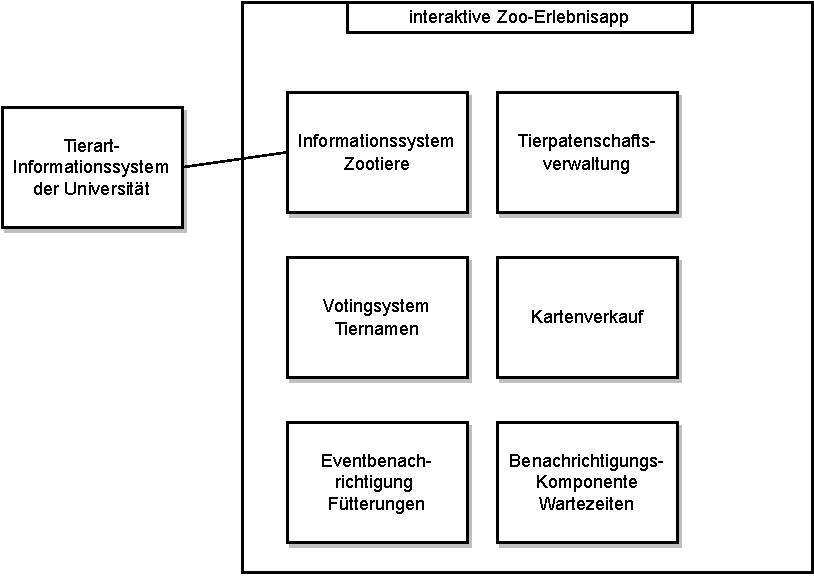
\includegraphics[width=0.7\textwidth]{Bilder/Kapitel-6/zoo_erlebnisapp.pdf}
	\caption{interaktive Zoo-Erlebnisapp}
	\label{fig:zoo_erlebnisapp}
\end{figure}

\textit{Ziele (erste Version):}
\begin{itemize}
	\item Alleinstellungsmerkmale des Zoos bekannt machen
	\item Steigende Besucherzahlen
	\item Zusätzliche Kooperationspartner gewinnen (Studiengänge, Schulen, Kindergärten, Bildungsprojekte) und Kooperationsprojekte akquirieren
\end{itemize}

\vspace{1em}

\textbf{Teilprojekt 2 „Softwaregestützte Automatisierung des Futterbestellprozesses“}

\textit{Stakeholder:} Tierpfleger, Lagerverwalter, Rechnungsabteilung der Zooverwaltung, IT-Abteilung des Zoos, ggf. weitere Abteilungen der Zooverwaltung, ggf. Futterlieferanten

\textit{Vision (erste Version):} Die überwiegend manuell ablaufenden Prozesse der Futterbestellung werden durch eine softwaregestützte Automatisierungslösung ersetzt. Die Tierpfleger haben wieder mehr Freiraum für ihre Fachaufgaben in der Versorgung der Tiere. Fehlerhafte Futterbestellungen werden verhindert. Das Futterbestellsystem wird an die Einkaufs- und Abrechnungssysteme der Zooverwaltung angebunden.

\textit{Ziele (erste Version):}
\begin{itemize}
	\item Die Tierpfleger von verwaltungstechnischen Aufgaben befreien
	\item Den Futterbestellprozess beschleunigen
	\item Den Futterbestellprozess zentralisieren
	\item Überblick über den Futterlagerbestand besitzen
	\item Minimierung der Futterentsorgung aufgrund überschrittener Haltbarkeiten
\end{itemize}


Herr Steiber: „Ich fasse nochmal zusammen. Wir konzentrieren uns in diesem Vorprojekt auf zwei Vorhaben \textit{Zoo-Erlebnisapp} und \textit{Softwaregestützte Automatisierung des Futterbestellprozesses}. Wir bilden zwei Teams, die parallel arbeiten. Sie, Frau Schwab, leiten das Teilprojekt 1 und Sie, Herr Fuller, übernehmen Teilprojekt 2. In beiden Teams werden kontinuierlich Domänenexpert:innen des Zoos vertreten sein. Es wird in den nächsten Tagen eine ihrer ersten Aufgaben sein, in Absprache mit Frau Dr. Walther die Domänenexpert:innen für die Teilprojekte festzulegen. Mit ersten Beschreibungen der Vorhaben haben wir heute begonnen. Das ist natürlich jetzt noch alles vage, für das erste Treffen aber schon ganz gut. Ich wünsche uns allen ein erfolgreiches weiteres Arbeiten!“